%\documentclass{article}
\documentclass[12pt, letterpaper, onecolumn]{article}
\usepackage[top=1.0in, bottom=1.0in, left=1.0in, right=1.0in]{geometry} %onecolumn

\usepackage[pdftex, colorlinks=true, filecolor=blue, urlcolor=blue]{hyperref}
\usepackage{amsmath,amsthm,amssymb}
\usepackage{graphicx}

\newcommand{\projname}{p5}
\newcommand{\projnum}{5}

%\input{common}
\newenvironment{packed_item}{
\begin{itemize}
  \setlength{\itemsep}{1pt}
  \setlength{\parskip}{0pt}
  \setlength{\parsep}{0pt}
}{\end{itemize}}

\begin{document}

\title{Formulating LCP for Articulated Rigid Bodies}
\author{}
% Jie did the derivation, so kasiu feels bad about being the author :(
\date{}
%\date{Last Edited: Spring 2012}

\maketitle
<<<<<<< HEAD
\section{Overview}
The following document describes the construction of the matrices responsible for solving LCP (linear-complimentarity problems) for articulated rigid bodies in generalized coordinates. The document assumes familiarity with the mathematical construction of LCP. This was originally intended as a guide for the implementation of the LCP solver for the DART dynamics library.
=======
\section{Introduction}
The following document describes the construction of the matrices responsible for contact handling for articulated rigid bodies in generalized coordinates. We formulate an implicit time-stepping, velocity-based LCP (linear-complementarity problem) to guarantee non-penetration, directional friction, and approximated Coulomb’s friction cone conditions, similar to Stewart and Trinkle \cite{Stewart:1996}. The document assumes familiarity with physics principles of frictional contact and the mathematical techniques for solving standard LCP. This was originally intended as a guide for the implementation of the LCP solver for the DART dynamics library.
>>>>>>> karen

\section{The Equations of Motion}
We begin our derivation from the following form of the equations of
motion for an articulated rigid body system with one contact point:
\begin{equation}
\label{eq:motionequations}
M(\vc{q})\ddot{\vc{q}} + C(\vc{q}, \dot{\vc{q}}) = \tau + J^T f_n \vc{n} + J^T
D \vc{f}_d
\end{equation}
\\
The terms of this equation are as follows:
\begin{packed_item}
\item $\vc{q}$: the state vector
\item $M$: the mass matrix
\item $C$: Coriolis, centrifugal, and gravitational forces
\item $\tau$: internal generalized forces
\item $J$: the Jacobian matrix evaluated at the contact point
\item $\vc{n}$: the normal force direction (Figure \ref{fig:example}(a))
\item $f_n$: the magnitude of the normal force
\item $D$: discretized friction cone bases (Figure \ref{fig:example}(a))
\item $\vc{f}_d$: the magnitudes of tangent forces along the discretized friction cone bases
\end{packed_item}

\begin{figure}
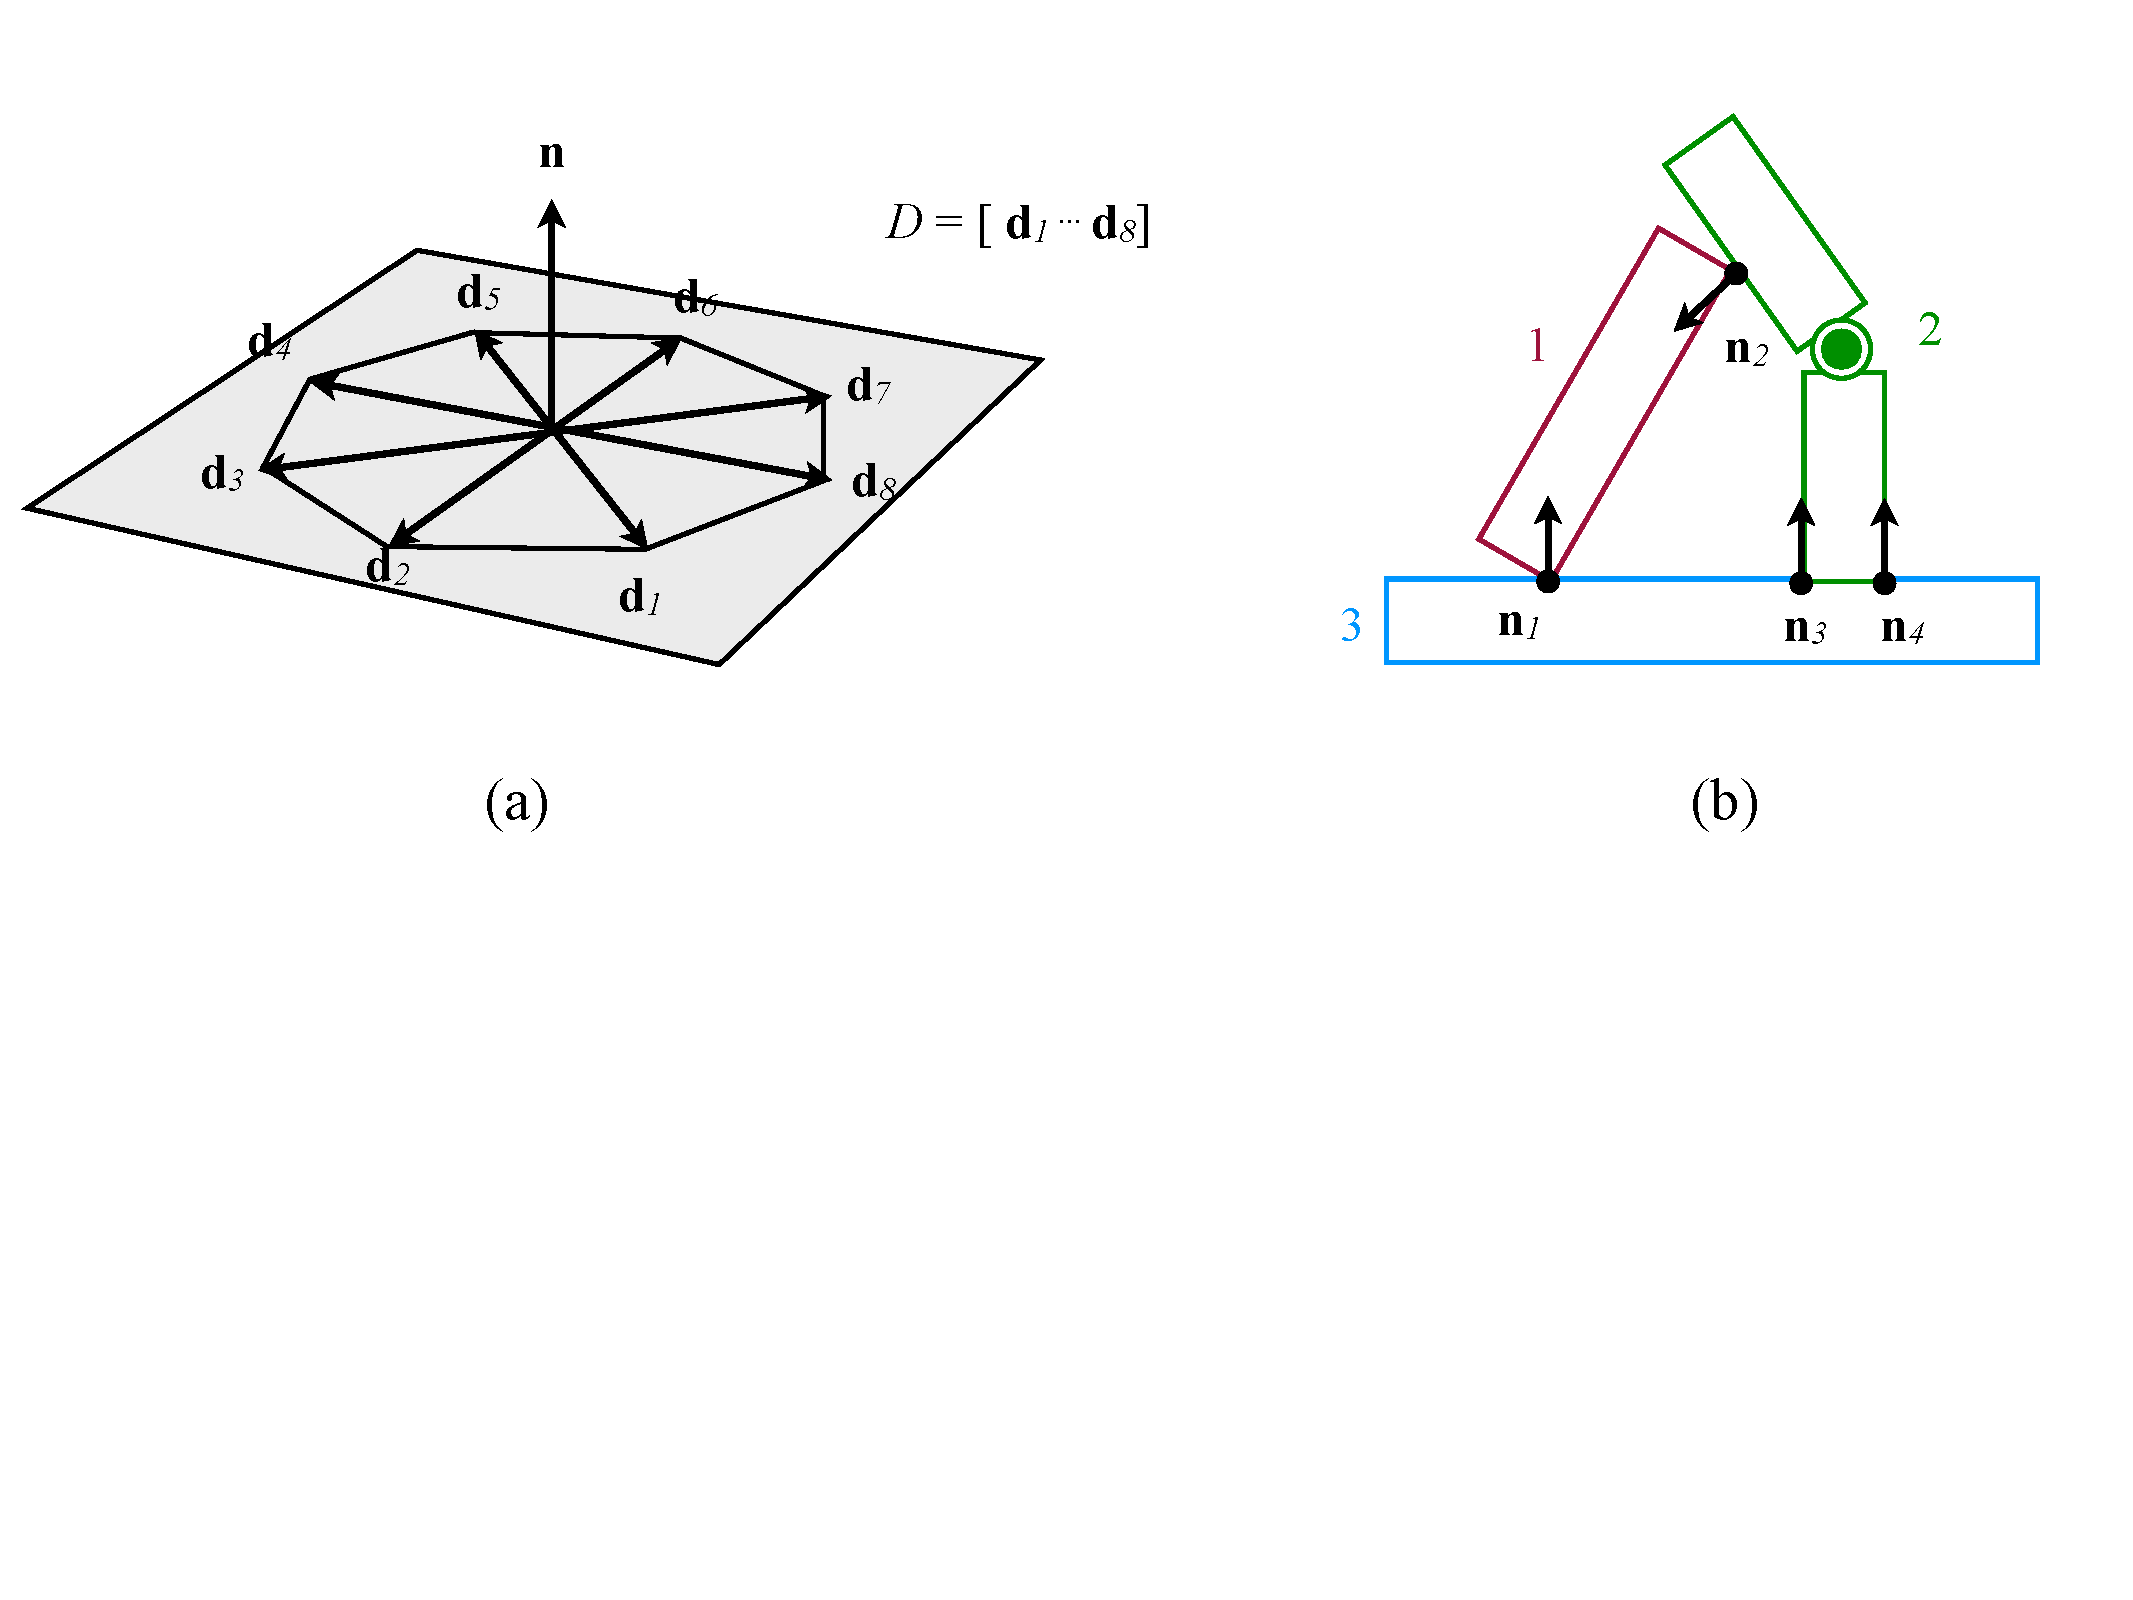
\includegraphics[width=6in]{example1.pdf}
\caption{An articulated system.}
\label{fig:example}
\end{figure}

We can discretize Equation \ref{eq:motionequations} as follows:
\begin{equation}
\label{eq:changemotionequations0}
M\ddot{\vc{q}} = M\frac{(\dot{\vc{q}}^{n+1}-\dot{\vc{q}}^n)}{\Delta{t}}
\end{equation}
\begin{equation}
\label{eq:changemotionequations1}
M\frac{(\dot{\vc{q}}^{n+1}-\dot{\vc{q}}^n)}{\Delta{t}} = -C(\vc{q}^n, \dot{\vc{q}}^n) + \tau^n + J^Tf_n\vc{n} + J^TD\vc{f}_d 
\end{equation}
\begin{equation}
\label{eq:changemotionequations2}
M\dot{\vc{q}}^{n+1} = M\dot{\vc{q}}^n - \Delta{t}(C(\vc{q}^n, \dot{\vc{q}}^n) - \tau^n) + \Delta{t}(J^Tf_n\vc{n} + J^TD\vc{f}_d)
\end{equation}
where superscripts $n$ and $n+1$ indicate the current and the next time
steps. In Equation \ref{eq:changemotionequations2} , the first two terms on the right are known values. 
We group these into a single term $\tau^*$:
\begin{equation}
\label{eq:taustar}
\tau^* = M\dot{\vc{q}}^n - \Delta{t}(C - \tau^n)
\end{equation}
We are then left with:
\begin{equation}
\label{eq:changemotionequations3}
M\dot{\vc{q}} = \tau^* + \Delta{t}(J^Tf_n\vc{n} + J^TD\vc{f}_d)
\end{equation}
where the unknown variables are the velocity of the state at the next time
step ($\dot{\vc{q}}$, superscript $n+1$ omitted for simplicity), the magnitude
of normal force ($f_n$), and the magnitudes of tangent forces ($\vc{f}_d$). 

Now let us consider the equations of motion for a more complex
situation shown in Figure \ref{fig:example}(b). There are four contact
points and three systems involved in the scene. We can stack the
equations of motion for each system in the following matrix form:

\begin{eqnarray}
\label{eq:changemotionequations4}
\left[\begin{matrix}M_1  & 0 & 0 \\ 0 & M_2 & 0 \\ 0 & 0 &
    M_3\end{matrix}\right]\left[\begin{matrix}\dot{q_1} \\ \dot{q_2}
    \\ \dot{q_3}\end{matrix}\right] = \left[\begin{matrix}{\tau_1}^*
    \\ {\tau_2}^* \\ {\tau_3}^*\end{matrix}\right] +
\Delta{t}\left[\begin{matrix}{J_{11}}^T\vc{n}_1 &
    {J_{12}}^T\vc{n}_2 & 0 & 0 \\ 0 & -J_{22}^T\vc{n}_2 & J_{23}^T
    \vc{n}_3 & J_{24}^T \vc{n}_4 \\ -J_{31}^T \vc{n}_1 & 0 & -J_{33}^T
    \vc{n}_3 & -J_{34}^T
    \vc{n}_4 \end{matrix}\right]\left[\begin{matrix}f_{n1} \\ f_{n2}
    \\ f_{n3} \\ f_{n4} \end{matrix}\right] \nonumber \\ +
\Delta{t}\left[\begin{matrix}J_{11}^T D_1 &
    J_{12}^TD_2 & 0 & 0 \\ 0 & -J_{22}^TD_2 & J_{23}^T
    D_3 & J_{24}^T D_4 \\ -J_{31}^T D_1 & 0 & -J_{33}^T
    D_3 & -J_{34}^T
    D_4 \end{matrix}\right]\left[\begin{matrix}\vc{f}_{d1} \\ \vc{f}_{d2} \\
    \vc{f}_{d3} \\ \vc{f}_{d4}\end{matrix}\right]
\end{eqnarray}
The subscript $i$ for $M_i$, $\dot{\vc{q}}_i$, and $\tau^*_i$ indicates the
$i$-th system, while the subscript $j$ for $\vc{n}_j$, $D_j$, $f_{nj}$,
and $\vc{f}_{dj}$ indicates the $j$-th contact. A Jacobian matrix
$J_{ij}$ has two subscripts indicating the Jacobian evaluated at
contact $j$ for the system $i$. 

For simplicity, we will rewrite some of these terms as matrices $N$ and $B$ as follows:
\begin{equation}
\label{eq:nbmatrix}
\begin{array}{cc}
N = \left[\begin{matrix}{J_{11}}^T\vc{n}_1 &
    {J_{12}}^T\vc{n}_2 & 0 & 0 \\ 0 & -J_{22}^T\vc{n}_2 & J_{23}^T
    \vc{n}_3 & J_{24}^T \vc{n}_4 \\ -J_{31}^T \vc{n}_1 & 0 & -J_{33}^T
    \vc{n}_3 & -J_{34}^T
    \vc{n}_4  \end{matrix}\right] \\
B = \left[\begin{matrix}J_{11}^T D_1 &
    J_{12}^TD_2 & 0 & 0 \\ 0 & -J_{22}^TD_2 & J_{23}^T
    D_3 & J_{24}^T D_4 \\ -J_{31}^T D_1 & 0 & -J_{33}^T
    D_3 & -J_{34}^T
    D_4 \end{matrix}\right]
\end{array}
\end{equation}
Assuming the total number of degrees of freedom for three systems is
$m$, the number of the contacts is $p$ ($p=4$ in Figure
\ref{fig:example}(b)), and the number of friction cone bases is $d$
($d = 8$ in Figure \ref{fig:example}(a)), the dimensions of $N$ and
$B$ are $m \times p$ and $m \times pd$, respectively. With these
substitutions, Equation \ref{eq:changemotionequations4} reduces to the
following:
\begin{equation}
\label{eq:changemotionequations5}
M\dot{\vc{q}} = \tau^* + \Delta{t} (N\vc{f}_n + B\vc{f}_d)
\end{equation}


\ignorethis{
At each time step, let $m$ denote the number of bodies in the system and $p$ denote the number of contact points.
For simplicity, we will ignore the time step superscripts ($n$) of the generalized coordinates $q$ and its derivatives.
\\
\\
Additionally, we use the notation $X_{ij}$ to describe a variable $X$, which corresponds to information about a contact between bodies $i$ and $j$.
For example, we would denote the normal $\vec{N}$ at the contact point between $i$ and $j$ as $\vec{N_{ij}}$.
\\
\\
We illustrate the following derivation using an example environment consisting of $(m = 3)$ rigid bodies in contact at $(c = 2)$ points. Without loss of generality, assume bodies 1 and 2 are in contact, and bodies 2 and 3 are in contact.
\\
\\
Using this example, we can rewrite Equation \ref{eq:changemotionequations3} as follows:
\begin{equation}
\label{eq:changemotionequations4}
\left[\begin{matrix}M_1  & 0 & 0 \\ 0 & M_2 & 0 \\ 0 & 0 & M_3\end{matrix}\right]\left[\begin{matrix}\dot{q_1} \\ \dot{q_2} \\ \dot{q_3}\end{matrix}\right] = \left[\begin{matrix}{\tau_1}^* \\ {\tau_2}^* \\ {\tau_3}^*\end{matrix}\right] + \Delta{t}\left[\begin{matrix}{J_{21}}^T\vec{N_{21}} & 0 \\ {J_{12}}^T\vec{N_{12}} & {J_{32}}^T\vec{N_{32}} \\ 0 & {J_{23}}^T\vec{N_{23}} \end{matrix}\right]\left[\begin{matrix}f_{n1} \\ f_{n2}\end{matrix}\right] + \Delta{t}\left[\begin{matrix}{J_{21}}^TD_{21} & 0 \\ {J_{12}}^TD_{12} & {J_{32}}^TD_{32} \\ 0 & {J_{23}}^TD_{23} \end{matrix}\right]\left[\begin{matrix}f_{d1} \\ f_{d2}\end{matrix}\right]
\end{equation}
For simplicity, we'll rewrite some of these terms as variables $N$ and $B$ as follows:
\begin{equation}
\label{eq:nbmatrix}
\begin{array}{cc}
N = \Delta{t}\left[\begin{matrix}{J_{21}}^T\vec{N_{21}} & 0 \\ {J_{12}}^T\vec{N_{12}} & {J_{32}}^T\vec{N_{32}} \\ 0 & {J_{23}}^T\vec{N_{23}} \end{matrix}\right] \\
B = \Delta{t}\left[\begin{matrix}{J_{21}}^TD_{21} & 0 \\ {J_{12}}^TD_{12} & {J_{32}}^TD_{32} \\ 0 & {J_{23}}^TD_{23} \end{matrix}\right]
\end{array}
\end{equation}
Note here that $N$ is a matrix, not to be confused with $N_{ij}$, which is a vector.
\\
\\
Also, we note that $N$ is a $(m^* \times c)$ matrix, instead of a full $(m^* \times 2c)$ matrix (as each contact corresponds to two normal vectors). This exploits the fact that $\vec{N_{ij}} = -\vec{N_{ij}}$ and that the magnitude of these vectors (forces) are the same. Thus, we can condense the matrix. Similarly, $B$ takes advantage of this as well. Here $m^*$ depends on both $m$, as well as the DOFs of each $q_i$. ($m^*$ is the product of $m$ and the respective number of DOFs for each $q_i$.)
\\
\\

With these substitutions, Equation \ref{eq:changemotionequations4} reduces to the following:
\begin{equation}
\label{eq:changemotionequations5}
M\dot{q} = \tau^* + N\vec{f_n} + B\vec{f_d}
\end{equation}
}
\section{LCP Formulation}
<<<<<<< HEAD
=======
The problem of contact handling is based on three types of
constraints: normal direction constraints, directional friction constraints,
and friction cone constraints. Together with equations of
motion described earlier, these three sets of constraints constitute a
LCP for unknown variables $\dot{\vc{q}}$, $\vc{f}_n$, $\vc{f}_d$, and
auxiliary variables $\lambda$.

\subsection{Normal Direction Constraints}
\begin{packed_item}
\item{expression 1:} $\vc{f}_n \geq 0$
\item{expression 2:} $N \dot{\vc{q}} \geq 0$
\item{expression 3:} $(N \dot{\vc{q}})^T\vc{f}_n = 0$
\end{packed_item}
Expression 1 ensures there is no pulling force. Expression 2 prevents
penetration by enforcing a nonnegative normal velocity at
contact. Expression 3 constrains the normal force based on the
velocity. If $N \dot{\vc{q}} > 0$, then $\vc{f}_n = 0$ (in
takeoff). If $\vc{f}_n > 0$ then $N \dot{\vc{q}} = 0$ (in contact).

\subsection{Directional Friction Constraints}
\begin{packed_item}
\item{expression 4:} $\vc{f}_d \geq 0$
\item{expression 5:} $B^T\dot{\vc{q}} + E\lambda \geq 0$
\item{expression 6:} $(B^T\dot{\vc{q}} + E\lambda)^T\vc{f}_d = 0$
\end{packed_item}
Here $E \in R^{pd \times p}$ is a binary matrix whose structure is
defined as follows: 
\begin{equation}
\label{eq:ematrix}
E = \left[\begin{matrix}\vc{e}_1 & & \\  & \ddots & \\  & & \vc{e}_p \end{matrix}\right]
\end{equation}
where $\vc{e}$ is a vector of ones in
$R^d$. Additionally, $\lambda$ is a vector in $R^p$ that contains all
of the auxiliary variables.
\begin{equation}
\label{eq:lambda}
\lambda = \left[\begin{matrix}\lambda_1 \\  \vdots \\ \lambda_p\end{matrix}\right]
\end{equation}

The goal of directional friction constraints is to ensure that contact
slipping on the surface is in the opposite direction of the friction
force. Let us first exam the first term of Expression 5,
$B^T\dot{\vc{q}}$, the velocity at contact projected onto each friction
cone basis vector. The projection will end up in one of the three cases:
\begin{enumerate}
\item The projected vector is closer to one of the bases than others. The most
  negative element in $B^T\dot{\vc{q}}$ is unique.
\item The projected vector is right in the middle of two basis
  vectors. The two most negative elements in $B^T\dot{\vc{q}}$ are the
  same.
\item The projected vector is a zero vector.
\end{enumerate}
Because the smallest possible value for any element
in $B^T\dot{\vc{q}} + E\lambda$ is zero (by Expression 5), the first case has at most
one zero element in $B^T\dot{\vc{q}} + E\lambda$. Assuming the index
of that zero element is $i$, Expression 5 and Expression 6 together
state that $\vc{f}_d$ must be a zero vector except for the $i$-th
element. This nonzero element in $\vc{f}_d$ determines the direction
of the friction force while the corresponding $i$-th element in
$B^T\dot{\vc{q}} + E\lambda$ indicates the most negative projection of
tangent velocity. Therefore, given a set of basis directions, the
friction force is indeed in the most opposite direction of contact
slipping. The second case rarely happens, but when it does we can
arbitrary pick one of the two bases to break the tie and apply the
same reasoning as the first case. The third case indicates either
static contact (when $\lambda = 0$) or contact breakage (when $\lambda
> 0$). It will be more clear after we introduce friction cone
constraints.

Is it valid to choose a large positive $\lambda$ such that all the
elements of $B^T\dot{\vc{q}} + E\lambda$ are greater than zero? It
does not seem to violate any of the expressions here, but we will see
the implication of that in the next subsection.

\ignorethis{
Assuming
there exists one zero element in $B^T\dot{\vc{q}} + E\lambda$ whose
index is $i$, the Expression 5 and Expression 6 together state that
$\vc{f}_d$ must be a zero vector except for the $i$-th element. This
nonzero element in $\vc{f}_d$ determines the direction of the friction
force. Since $B^T\dot{\vc{q}}$ is the velocity at contact projected
onto friction cone bases, the $i$-th element of $B^T\dot{\vc{q}} +
E\lambda$ indicates the most negative projection of tangent
velocity. Therefore, given a set of basis directions, the friction
force is indeed in the most opposite direction of contact slipping. Is
it valid to choose a large positive $\lambda$ such that all the
elements of $B^T\dot{\vc{q}} + E\lambda$ are greater than zero? The
answer is no but to see that we need to also consider friction cone
constraints.}

\subsection{Friction Cone Constraints}
\begin{packed_item}
\item{expression 7:} $\lambda \geq 0$
\item{expression 8:} $\mu\vc{f}_n - E^T\vc{f}_d \geq 0$
\item{expression 9:} $\lambda^T(\mu\vc{f}_n - E^T\vc{f}_d) = 0$
\end{packed_item}
Friction cone constraints describe the switch condition between static
state and slipping state of a contact. From the previous section, we
know that at most one element of $\vc{f}_d$ can be nonzero for the first (and
the second) case. Therefore, Expression 8 states that the ratio of tangent
contact force to normal contact force must be less than or equal to
the friction coefficient $\mu$. If the contact force is within the
friction cone (inequality case in Expression 8), $\lambda$ must be
zero by Expression 9. When $\lambda$ is zero, the corresponding
Expression 5 becomes $B^T\dot{\vc{q}} \geq 0$. Because the bases of
friction cones are arranged in pairs of opposite directions (\eg
$\vc{d}_1 = -\vc{d}_5$, $\vc{d}_2 = -\vc{d}_6$), the only way for all
elements to be nonnegative is when $B^T\dot{\vc{q}}$ is a zero vector
(no slipping), hence the friction cone condition.

Now, we can go back to the question about validity of selecting a
large positive $\lambda$ such that all the elements of
$B^T\dot{\vc{q}} + E\lambda$ are greater than zero. If we do so,
$\vc{f}_d$ will be all zeros by Expression 6, which leads to
$\mu\vc{f}_n \geq 0$ by Expression 8. If $\vc{f}_n > 0$, $\lambda$
must be zero by Expression 9, contradicting the assumption that
$\lambda$ is a large positive value. Therefore, $B^T\dot{\vc{q}} +
E\lambda$ can be greater than zero only when the contact is broken
($\vc{f}_n = 0$). As long as the contact exists, $\lambda$ will always
be either zero or a positive value that makes the most negative
element of $B^T\dot{\vc{q}} + E\lambda$ exactly zero.

\ignorethis{
 Recall that at most one element
of $\vc{f}_d$ can be nonzero when $B^T\dot{\vc{q}} + E\lambda$ is not
a zero vector \footnote{In a special case when the tangent velocity is
  right in the middle of two basis directions, there are two nonzero
  elements in $\vc{f}_d$. We can arbitrarily pick one of the two
  bases.}. Therefore, Expression 8 states that the ratio of tangent
contact force to normal contact force must be less than or equal to
the friction coefficient $\mu$. If the contact force is within the
friction cone (inequality case in Expression 8), $\lambda$ must be
zero by Expression 9. When lambda is zero, the corresponding
Expression 5 becomes $B^T\dot{\vc{q}} \geq 0$. Because the bases of
friction cones are arranged in pairs of opposite directions (\eg
$\vc{d}_1 = -\vc{d}_5$, $\vc{d}_2 = -\vc{d}_6$), the only way for all
elements to be nonnegative is when $B^T\dot{\vc{q}}$ is a zero vector
(no slipping), hence the friction cone condition.

Now, we can go back to the question about validity of selecting a large positive
$\lambda$ such that all the elements of $B^T\dot{\vc{q}} + E\lambda$
are greater than zero. If we do so, $\vc{f}_d$ will be all zeros by
Expression 6. Consequently,
Expression 8 becomes $\mu\vc{f}_n -
E^T\vc{f}_d > 0$, which leads to $\lambda = 0$ by Expression 9. This
contradicts our assumption that $\lambda$ is a large positive
value. Therefore, if we consider all the constraints together,
$\lambda$ will always be either zero or a positive value that makes
the most negative element of $B^T\dot{\vc{q}} + E\lambda$ exactly
zero.}

\subsection{LCP}
Putting all the constraints together, we can construct the following linear system of equations:
\begin{equation}
\label{eq:bigsystem}
\begin{array}{cc}
\left[\begin{matrix}0 \\\vc{a} \\ \vc{b} \\ \vc{c} \end{matrix}\right] =
\left[\begin{matrix}M & -\Delta t N & -\Delta t B & 0 \\ N^T & 0 & 0 & 0 \\ B^T & 0 & 0 & E \\ 0 & \mu & -E^T & 0\end{matrix}\right]\left[\begin{matrix}\vc{\dot{\vc{q}}} \\ \vc{f}_n \\ \vc{f}_d \\ \lambda\end{matrix}\right] + \left[\begin{matrix}-\tau^* \\ 0 \\ 0 \\0\end{matrix}\right] \\
\begin{matrix}
\left[\begin{matrix}\vc{f}_n \\ \vc{f}_d \\ \lambda\end{matrix}\right] \geq 0, & 
\left[\begin{matrix}\vc{a} \\ \vc{b} \\ \vc{c}\end{matrix}\right] \geq 0, &
\left[\begin{matrix}\vc{a} \\ \vc{b} \\ \vc{c}\end{matrix}\right]^T\left[\begin{matrix}\vc{f}_n \\ \vc{f}_d \\ \lambda\end{matrix}\right] = 0
\end{matrix}
\end{array}
\end{equation}
The first row of the system is based on Equation
\ref{eq:changemotionequations5}. The remaining three rows, as well as
the constraints, encapsulate the nine LCP conditions described
above. Unfortunately, the construction described is in MLCP (Mixed
LCP) form. To convert it to standard form, we need to make a few
adjustments.

\ignorethis{
\section{LCP Formulation}
>>>>>>> karen
Recall that we need $V_n$ (the relative velocity), which is given by the following expression:
\begin{equation}
\label{eq:vn0}
V_n = N^T\dot{q}
\end{equation}
Expanding this out using the example problem yields the following:
\begin{equation}
\label{eq:vn1}
V_n = \left[\begin{matrix}\vec{N_{21}}^TJ_{21} & \vec{N_{12}}^TJ_{12} & 0 \\ 0 & \vec{N_{32}}^TJ_{32} & \vec{N_{23}}^TJ_{23}\end{matrix}\right]\left[\begin{matrix}\dot{q_1} \\ \dot{q_2} \\ \dot{q_3}\end{matrix}\right]
\end{equation}
\begin{equation}
\label{eq:vn2}
V_n = \left[\begin{matrix}\vec{N_{21}}^TJ_{21}\dot{q_1} + \vec{N_{12}}^TJ_{12}\dot{q_2} \\ \vec{N_{32}}^TJ_{32}\dot{q_2} + \vec{N_{23}}^TJ_{23}\dot{q_3}\end{matrix}\right]
\end{equation}
Since $\vec{N_{ij}} = -\vec{N_{ji}}$, we can reduce this further:
\begin{equation}
\label{eq:vn3}
V_n = \left[\begin{matrix}\vec{N_{21}}^T(J_{21}\dot{q_1} - J_{12}\dot{q_2}) \\ \vec{N_{32}}^T(J_{32}\dot{q_2} - J_{23}\dot{q_3})\end{matrix}\right]
\end{equation}

\subsection{Normal Direction Constraints}
We now begin revisiting the constraints for LCP.
\begin{packed_item}
\item $\vec{f_n} \geq 0$
\item $\vec{v_n} \geq 0$
\item $\vec{v_n}^T\vec{f_n} = 0$
\end{packed_item}
The first expression ensures there is no pulling force. The second expression prevents penetration with the contact surface. The third expression constrains the normal force based on the velocity. If $\vec{v_n} > 0$, then $\vec{f_n} = 0$ (in takeoff). If $\vec{v_n} = 0$, then $\vec{f_n} \geq 0$ (in contact).

\subsection{Friction Cone Constraints}
\begin{packed_item}
\item $\vec{\lambda} \geq 0$
\item $\mu\vec{f_n} - E^T\vec{f_d} \geq 0$
\item $\lambda(\mu\vec{f_n} - E^T\vec{f_d}) = 0$
% Should this be \vec{lamba}?
\end{packed_item}
Here $E$ is a $(cd \times c)$ matrix where $d$ is the number of contact (friction cone) directions and $c$ is the number of contacts (as defined above). As an example, the structure of $E$ for a problem with $(d = 3)$ contact directions and $(c = 2)$ contacts would be as follows:
\begin{equation}
\label{eq:ematrix}
E = \left[\begin{matrix}1 & 0 \\ 1 & 0 \\ 1 & 0 \\ 0 & 1 \\ 0 & 1 \\ 0 & 1\end{matrix}\right]
\end{equation}
Additionally, $\vec{\lambda}$ is a vector of length $c$ that contains all of the $\lambda$ values.
\begin{equation}
\label{eq:lambda}
\vec{\lambda} = \left[\begin{matrix}\lambda_1 \\ \lambda_2 \\ .. \\ \lambda_c\end{matrix}\right]
\end{equation}

\subsection{Directional Friction Constraints}
\begin{packed_item}
\item $\vec{f_d} \geq 0$
\item $B^T\dot{q} + E\vec{\lambda} \geq 0$
\item $(B^T\dot{q} + E\vec{\lambda})^T\vec{f_d} = 0$
\end{packed_item}
From this, we can construct the following linear system of equations:
\begin{equation}
\label{eq:bigsystem}
\begin{array}{cc}
\left[\begin{matrix}0 \\ a \\ b \\ c \end{matrix}\right] = \left[\begin{matrix}M & -N & -B & 0 \\ N^T & 0 & 0 & 0 \\ B^T & 0 & 0 & E \\ 0 & \mu & -E^T & 0\end{matrix}\right]\left[\begin{matrix}\vec{\dot{q}} \\ \vec{f_n} \\ \vec{f_d} \\ \vec{\lambda}\end{matrix}\right] + \left[\begin{matrix}-\tau^* \\ 0 \\ 0 \\0\end{matrix}\right] \\
\begin{matrix}
\left[\begin{matrix}\vec{f_n} \\ \vec{f_d} \\ \vec{\lambda}\end{matrix}\right] \geq 0, & 
\left[\begin{matrix}a \\ b \\ c\end{matrix}\right] \geq 0, &
\left[\begin{matrix}a \\ b \\ c\end{matrix}\right]^T\left[\begin{matrix}\vec{f_n} \\ \vec{f_d} \\ \vec{\lambda}\end{matrix}\right] = 0
\end{matrix}
\end{array}
\end{equation}
The first row of the system is based on Equation \ref{eq:changemotionequations5}. The remaining three rows, as well as the constraints, encapsulate the nine LCP conditions described above.
\\
\\
Here $(a, b, c)$ are the results of the following constraints: 
\begin{packed_item}
\item $\vec{v_n} \geq 0$
\item $\mu\vec{f_n} - E^T\vec{f_d} \geq 0$
\item $B^T\dot{q} + E\vec{\lambda} \geq 0$
\end{packed_item}
The expression for $\vec{v_n}$ comes from solving for the relative velocity in Equation \ref{eq:vn3}.
\\
\\
<<<<<<< HEAD
Unfortunately, the construction described is in MLCP (Mixed LCP) form. To convert it to standard form, we need to make a few adjustments.
=======
Unfortunately, the construction described is in MLCP (Mixed LCP)
form. To convert it to standard form, we need to make a few
adjustments.
}
>>>>>>> karen

\section{Standard LCP Form}
<<<<<<< HEAD
Standard LCP is of the following form:
\begin{equation}
\begin{array}{cc}
\vec{w} = A\vec{z} + \vec{q} \\
\vec{w} \geq 0 \\
\vec{z} \geq 0 \\
\vec{w}^T\vec{z} = 0
\end{array}
\end{equation}
If we solve for $\dot{q}$, we get:
\begin{equation}
\dot{q} = M^{-1}(V\vec{f_n} + B\vec{f_d} + \tau^*)
\end{equation}
We can then reorder Equation \ref{eq:bigsystem} slightly to get the following:
\begin{equation}
\label{eq:slcp0}
\left[\begin{matrix}a \\ b \\ c\end{matrix}\right] = \left[\begin{matrix}N^TM^{-1}N & N^TM^{-1}B & 0 \\ B^TM^{-1}N & B^TM^{-1}B & E \\ \mu & -E^T & 0\end{matrix}\right]\left[\begin{matrix}\vec{f_n} \\ \vec{f_d} \\ \vec{\lambda}\end{matrix}\right] + \left[\begin{matrix}N^TM^{-1}\tau^* \\ B^TM^{-1}\tau^* \\ 0\end{matrix}\right]
\end{equation}
Where:
\begin{equation}
\label{eq:slcp1}
\begin{array}{cc}
\vec{w} = \left[\begin{matrix}a \\ b \\ c\end{matrix}\right] \\
A = \left[\begin{matrix}N^TM^{-1}N & N^TM^{-1}B & 0 \\ B^TM^{-1}N & B^TM^{-1}B & E \\ \mu & -E^T & 0\end{matrix}\right] \\
\vec{z} = \left[\begin{matrix}\vec{f_n} \\ \vec{f_d} \\ \vec{\lambda}\end{matrix}\right] \\
\vec{q} = \left[\begin{matrix}N^TM^{-1}\tau^* \\ B^TM^{-1}\tau^* \\ 0\end{matrix}\right]
\end{array}
\end{equation}
Once we have $\vec{w}$ and $\vec{z}$, we can plug values back into the equations of motion to get $\dot{q}^{n + 1}$.
=======
The standard LCP solves for two vectors $\vc{w}$ and $\vc{z}$, and is of the following form:
\begin{equation}
\begin{array}{cc}
\vc{w} = A\vc{z} + \vc{q} \\
\vc{w} \geq 0 \\
\vc{z} \geq 0 \\
\vc{w}^T\vc{z} = 0
\end{array}
\end{equation}
If we express $\dot{\vc{q}}$, as $\dot{\vc{q}} = M^{-1}(\Delta t
N\vc{f}_n + \Delta t B\vc{f}_d + \tau^*)$, we can then reorder Equation \ref{eq:bigsystem} slightly to get the following:
\begin{equation}
\label{eq:slcp0}
\left[\begin{matrix}\vc{a} \\ \vc{b} \\ \vc{c}\end{matrix}\right] =
\left[\begin{matrix}\Delta t N^TM^{-1}N & \Delta t N^TM^{-1}B & 0 \\ \Delta t B^TM^{-1}N & \Delta t B^TM^{-1}B & E \\ \mu & -E^T & 0\end{matrix}\right]\left[\begin{matrix}\vc{f}_n \\ \vc{f}_d \\ \lambda\end{matrix}\right] + \left[\begin{matrix}N^TM^{-1}\tau^* \\ B^TM^{-1}\tau^* \\ 0\end{matrix}\right]
\end{equation}
where:
\begin{equation}
\label{eq:slcp1}
\begin{array}{cc}
\vc{w} = \left[\begin{matrix} \vc{a} \\ \vc{b} \\ \vc{c}\end{matrix}\right] \\
A = \left[\begin{matrix}\Delta t N^TM^{-1}N & \Delta t N^TM^{-1}B & 0 \\ \Delta t B^TM^{-1}N & \Delta t B^TM^{-1}B & E \\ \mu & -E^T & 0\end{matrix}\right] \\
\vc{z} = \left[\begin{matrix}\vc{f}_n \\ \vc{f}_d \\ \lambda\end{matrix}\right] \\
\vc{q} = \left[\begin{matrix}N^TM^{-1}\tau^* \\ B^TM^{-1}\tau^* \\ 0\end{matrix}\right]
\end{array}
\end{equation}

We can now solve this standard LCP using any LCP solver, such as
Lemke's algorithm. Once we have $\vc{w}$ and $\vc{z}$, we can discard
$\vc{w}$ and plug values in $\vc{z}$ back into the equations of motion
to get $\dot{\vc{q}}^{n + 1}$.
>>>>>>> karen

\end{document}